\section{Summary Statistics}

In Simulation-Based Inference (SBI), the choice of summary statistics $S(y)$ is critical as it determines the amount of information extracted from high-dimensional raw data \parencite{beaumont2002approximate}.
In this section, we describe the systematic process used to identify a set of informative features that resolve parameter non-identifiability.

\subsection{The Identification Challenge: The $\beta$-$\rho$ Trade-off}

Initial experiments using basic summary statistics revealed a significant "ridge" in the joint posterior distribution of the infection rate $\beta$ and the rewiring rate $\rho$.
This ridge suggests an equifinality problem where a high-infection/high-rewiring scenario and a low-infection/low-rewiring scenario produce similar overall infection scales.
The model struggles to distinguish between a virus that spreads rapidly but is countered by fast network adaptation, and a virus that spreads slowly in a more stable network \parencite{demirel2017dynamics}.
To resolve this, we performed a comparative simulation analysis between parameter sets at both ends of the observed ridge.
Figure \ref{fig:sir_comparison} illustrates the distinct temporal dynamics of these cases, suggesting that peak timing and structural network changes are key to decoupling these parameters.

\begin{figure}[H]
    \centering
    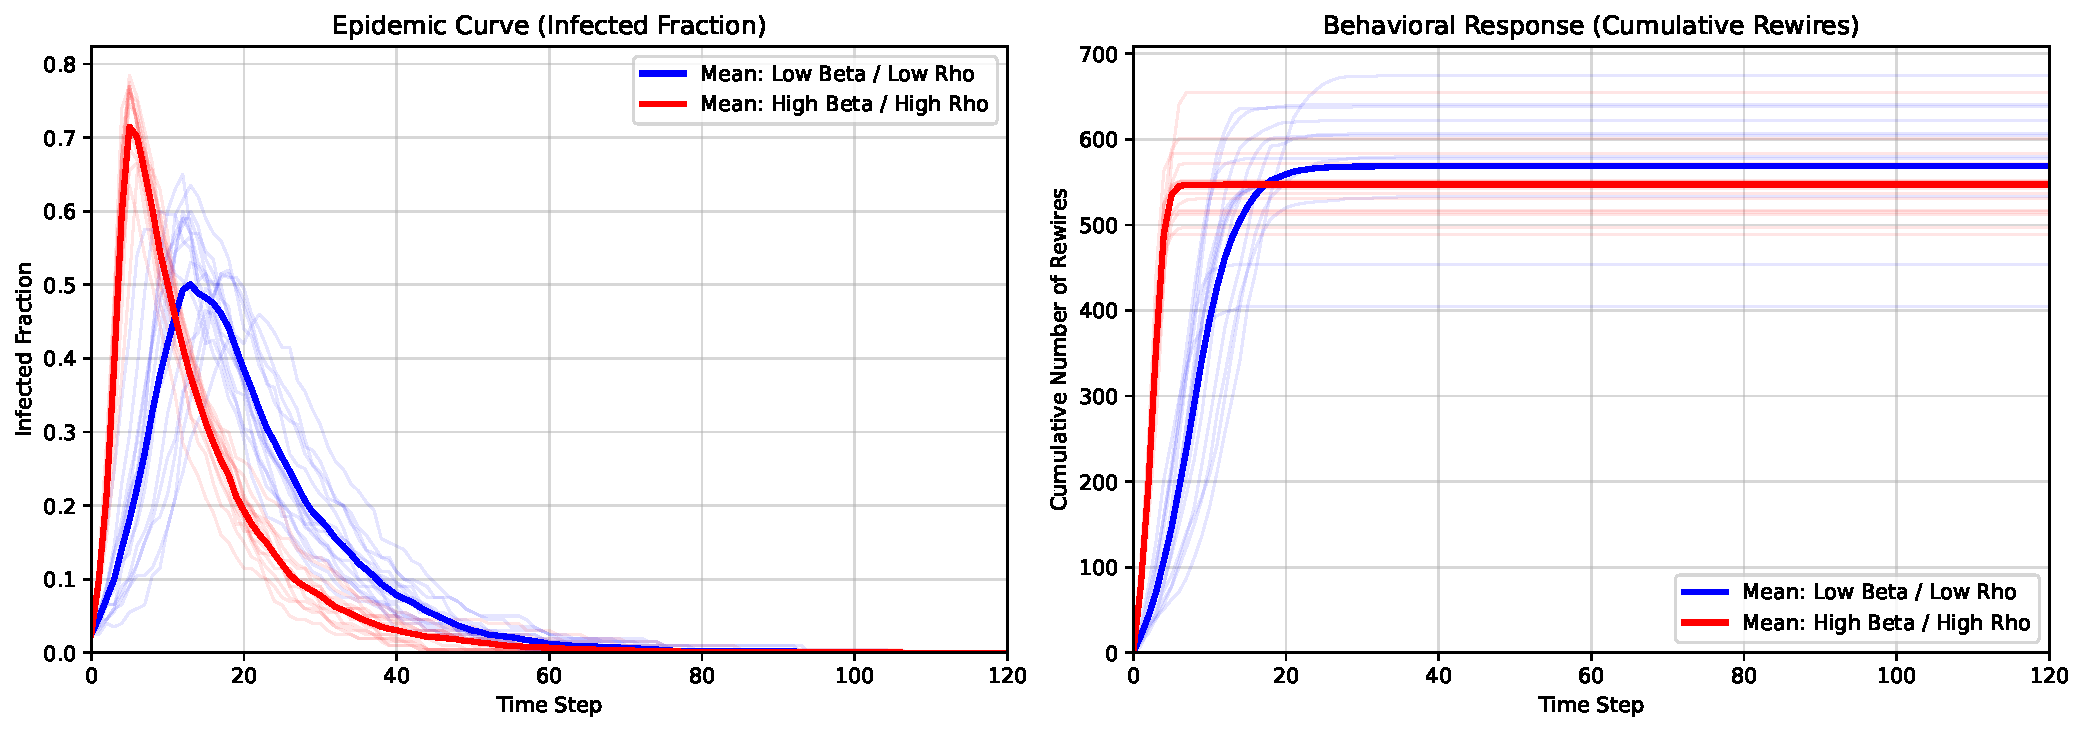
\includegraphics[width=0.9\textwidth]{plots/smc_abc_SIR_plot_1.pdf}
    \caption{Comparison of SIR dynamics and rewiring behavior for High $\beta$/High $\rho$ versus Low $\beta$/Low $\rho$ scenarios.}
    \label{fig:sir_comparison}
\end{figure}

\subsection{Selection of Informative Features}

Based on the observed dynamics, we expanded our summary statistic vector to five dimensions to capture both temporal and topological information:

\begin{itemize}
    \item \textbf{$s_1$: Peak Infected Fraction}: Captures the maximum intensity of the outbreak.
    \item \textbf{$s_2$: Log Rewire-to-Infection Ratio}: Measures the efficiency of behavioral response relative to the total infection risk.
    \[ s_2 = \log \left( \frac{\sum_{t} R_t}{\sum_{t} I_t + \epsilon_{small}} \right) \]
    \item \textbf{$s_3$: Log Final Degree Variance}: Detects the topological "scars" left by the rewiring process on the network structure.
    \item \textbf{$s_4$: Log Weighted Infection Timing}: Captures the "center of mass" of the epidemic curve, providing a robust metric for peak timing.
    \[ s_4 = \log \left( \frac{\sum_{t} t \cdot I_t}{\sum_{t} I_t} \right) \]
    \item \textbf{$s_5$: Log Maximum Step Rewire Rate}: Captures the burstiness of the behavioral response.
\end{itemize}

While these statistics are highly informative, they exhibit significant internal correlations.
A naive Euclidean distance fails to account for this dependent structure, which necessitates the use of a more sophisticated distance metric.
The implementation of the Mahalanobis distance to address these correlations is detailed in Section 4.2.

% \subsection{Distance Metric: Mahalanobis Distance}

% Because these statistics are inherently correlated (e.g., peak height and timing), a naive Euclidean distance is suboptimal. 
% In our final SMC-ABC implementation, we employ the Mahalanobis distance:
% \begin{equation}
%     d(s, s_{obs}) = \sqrt{(s - s_{obs})^T \mathbf{\Sigma}^{-1} (s - s_{obs})}
% \end{equation}
% where $\mathbf{\Sigma}$ is the covariance matrix estimated from the observed replicates. 
% This approach decorrelates the summary statistics and ensures that the inference process is sensitive to the unique information provided by each feature, effectively breaking the $\beta$-$\rho$ ridge.